\synctex=1
\documentclass[12pt]{article}
%Import geometry for smaller top
\usepackage{geometry}
% Required for inserting images
\usepackage{graphicx}
\graphicspath{{./images/}}
%Header and footer
\usepackage{fancyhdr}
%Language setting
\usepackage[utf8]{inputenc}
\usepackage[T2A]{fontenc}
\usepackage[russian]{babel}
%For better list
\usepackage{enumitem}
%For correct math operation
\usepackage{amsmath}
\usepackage{hyperref}
\usepackage{amsfonts}
\usepackage{booktabs}
\usepackage{amssymb}

\geometry{a4paper,
 total={170mm,257mm},
 left=20mm,
 top=30mm,
 bottom=25mm
}

\fancypagestyle{first style}
{
\chead{\footnotesize{Санкт-Петербургский Национальный Исследовательский Университет ИТМО\\Факультет Технологического Менеджмента и Инноваций}}
\cfoot{\footnotesize{Санкт-Петербург 2025г.}}
\renewcommand{\headrulewidth}{0pt}
}

\begin{document}

\pagestyle{fancy}
$\thispagestyle{first style}$

\centering{
\includegraphics[scale=0.5]{LogoITMO}}

\vspace{25mm}

\centering{Вариант №24\\Лабораторная Работа №3\\По дисциплине\\Математическая статистика}

\vspace{50mm}

\begin{flushright}
Выполнила студентка группы U3275:\\Савинова Алина Константиновна\\
\vspace{5mm}
Преподаватель:\\Кожевникова Элина Олеговна\\
\end{flushright}

\newpage

\pagestyle{empty}
\raggedright

\section{Обработка выборки A}

Выборка: 7, 11, 5, 5, 5, 5, 9, 4, 5, 3, 8, 5, 3, 8, 3,
11, 3, 9, 6, 8, 3, 3, 6, 2, 7, 4, 4, 3, 5, 7,
4, 6, 5, 2, 9, 5, 8, 6, 1, 1, 7, 7, 4, 4, 9,
7, 4, 3, 1, 6, 6, 4, 5, 4, 5, 5, 7, 8, 6, 8,
4, 10, 2, 7, 7, 5, 9, 6, 11, 2, 7, 7, 9, 2, 6, 8.

\subsection{Проверка гипотез о распределении (критерий Пирсона)}

\subsubsection*{Гипотеза 1: Распределение Пуассона}
Распределение Пуассона записывается, как мы ранее обозначили, следующим образом $X \sim Pois(\lambda)$, соответственно у него будут следующие значения характеристик и параметров:\\
Параметр: $\hat{\lambda} = \bar{x} = 5.605$; Объём выборки: $n = 76$; Уровень значимости: $\alpha = 0.05$\\

\begin{table}[h]
\begin{tabular}{ |c|c|c|c|c|c| }
\hline
$x_i$ & $n_i$ & $p_i$ & $np_i$ & $\frac{(n_i - np_i)^2}{np_i}$ \\
\hline
1-2 & 8 & 0.0784 & 5.9588 & 0.6992 \\
\hline
3 & 8 & 0.1080 & 8.2057 & 0.0051 \\
\hline
4 & 10 & 0.1513 & 11.4988 & 0.1953 \\
\hline
5 & 13 & 0.1696 & 12.8907 & 0.0009 \\
\hline
6 & 9 & 0.1585 & 12.0427 & 0.7687 \\
\hline
7 & 11 & 0.1269 & 9.6432 & 0.1909 \\
\hline
8 & 7 & 0.0889 & 6.7566 & 0.0088 \\
\hline
9+ & 6 & 0.1148 & 8.7240 & 0.1866 \\
\hline
\end{tabular}
\centering
\caption{Расчёт критерия $\chi^2$ для распределения Пуассона}
\end{table}
\vspace{5mm}

Мы рассчитывали вероятности по уже известной нам формуле: $P(X = k) = \frac{(\lambda^k * e^{(-\lambda)})}{k!}$

На основе данных, которые мы выше определили мы теперь можем найти и записать нашу $\chi^2$ стистику. Давайте найдем ее:
\[
\chi^2_{\text{набл}} = \sum \frac{(n_i - np_i)^2}{np_i} = 2.0557
\]
В нашем случае число степеней свободы будет: $k = 8$, а также у нас имеется оцененный параметр $r = 1$, который пригодится нам в рассчете критического значения 
(небольшое пояснение: $k$ - число интервалов группировки после объединения, $l$ - число параметров предполагаемого распределения, в нашем случае у нас один параметр для распределения Пуассона).
Давайте же для начала найдем значение для нахождения критического:
$df = k - r - 1 = 6$ \\
Теперь мы подставляем это число в $\chi^2$ и не забываем учитывать нашу $\alpha$:\\
$$\chi^2_{0.95}(6) = 12.5916$$
Так мы получили наше критическое значение и теперь можем сделать вывод на основе него, если наше наблюдаемое меньше критического значения, то мы принимаем (или еще говорят, НЕ отвергаем) гипотезу $H_0$.
$\chi^2_{\text{набл}} = 2.0557 < 12.5916 \Rightarrow$ \textbf{гипотеза $H_0$ не отвергается}.\\
\vspace{10mm}
Также можем обратиться к графику и наглядно посмотреть:
\begin{figure}[h]
\centering
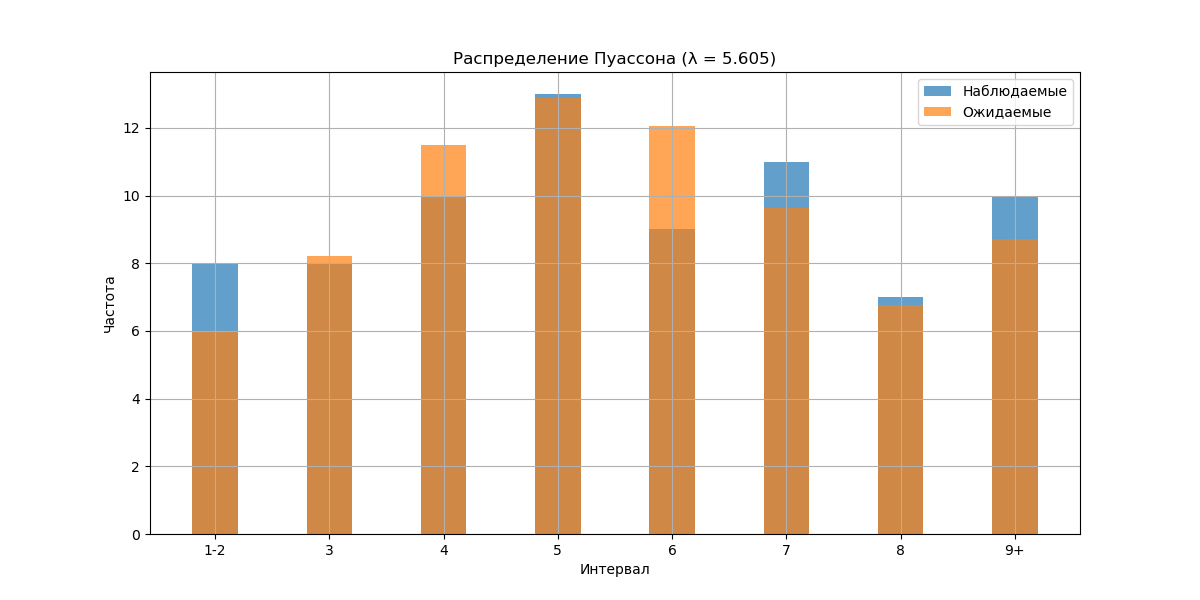
\includegraphics[scale=0.5]{pois.png}
\caption{График сравнения для распределения Пуассона}    
\end{figure}

\subsubsection*{Гипотеза 2: Биномиальное распределение}
Биноминальное распределение мы записываем как $X \sim Bin(n,p)$ и в нашем случае, мы уже знаем значения этих параметров: $n = 11$, $\hat{p} = 0.518$ \\
Тогда давайте составим таблицу с вероятностями распределения:
\begin{table}[h]
\centering
\begin{tabular}{ |c|c|c|c|c|c| }
\hline
$x_i$ & $n_i$ & $p_i$ & $np_i$ & $\frac{(n_i - np_i)^2}{np_i}$ \\
\hline
0-3 & 16 & 0.0917 & 6.9705 & 11.6969 \\
\hline
4 & 10 & 0.1436 & 10.9138 & 0.0765 \\
\hline
5 & 13 & 0.2161 & 16.4205 & 0.7125 \\
\hline
6 & 9 & 0.2322 & 17.6469 & 4.23697 \\
\hline
7 & 11 & 0.1782 & 13.5464 & 0.4787 \\
\hline
8-11 & 17 & 0.1382 & 10.5019 & 4.0207 \\
\hline
\end{tabular}
\caption{Расчёт критерия $\chi^2$ для биномиального распределения}
\end{table}

Теперь мы также как и вы предыдущем пункте рассчитаем наблюдаемую статистику $\chi^2$, а после рассчитаеми сравним с критическим значением:
\[
\chi^2_{\text{набл}} = 25.182
\]
Снова рассчитаем число степеней свободы: $df = 6 - 2 - 1 = 3$ 
Вновь рассчитаем критическое значение не забывая про $\alpha$ и подставим наше число степеней свободы: $\chi^2_{0.95}(3) = 7.8147$ \\
Сравним и сделаем вывод относительно нашей гипотезы $H_0$: $\chi^2_{\text{набл}} = 25.182 > 9.488 \Rightarrow$ \textbf{гипотеза $H_0$ отвергается}.

Мы также можем обратиться к графику и наглядно сравнить:
\begin{figure}[h]
\centering
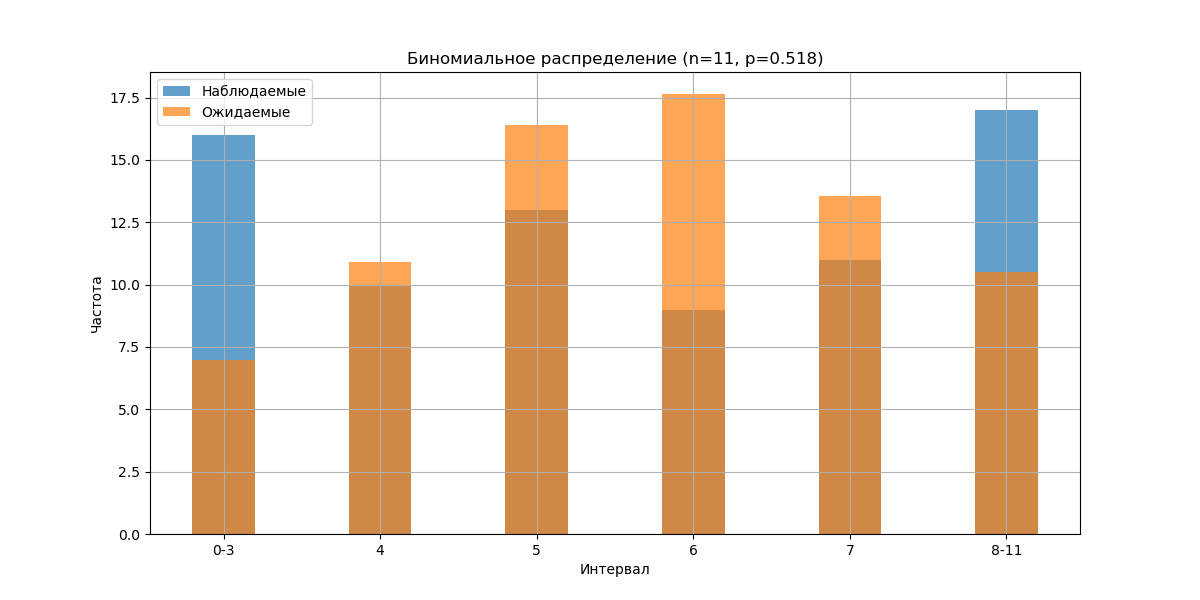
\includegraphics[scale=0.5]{binominal.png}
\caption{График сравнения для биномиального распределения}    
\end{figure}

\subsection{Вывод о наилучшем распределении}
Распределение Пуассона лучше соответствует данным, так как:
\begin{itemize}
    \item Гипотеза не отвергнута ($p > 0.05$)
    \item Теоретические частоты лучше соответствуют наблюдаемым
    \item Биномиальное распределение отвергнуто из-за значительного расхождения частот
\end{itemize}

\subsection{Проверка гипотезы о неизвестном среднем}
Давайте для начала выдвинем гипотезу и не забудем, что в условии задания мы будем брать $a_0$ как: $a_0 = [\overline{x}] + 0.5 = 5.5$:\\
$$H_0: a = a_0$$
Тогда наши параметры будут принимать значения, мы ранее уже их вычисляли:
$\bar{x} = 5.605$, $s^2 = 6.027$, $s = 2.455$, $n = 76$ \\
Тогда давайте вычислим нашу статистику, обозначим ее за $z$ (так принято обозначать и мы не будем отходить от общепринятых практик):
\[
z = \frac{\bar{x} - a_0}{s/\sqrt{n}} = \frac{5.605 - 5.5}{2.455/\sqrt{76}} \approx 0.3737
\]
Для вычисления критической области используется следующее неравенство из которого его можно найти искомое нами значение:
$$|z| > z_{1-\alpha/2} \approx 1.96$$
И уже на основе этих данных мы можем сделать выводы о нашей предложенной гипотезе, если наша $Z$-статистика окажется меньше чем критическая область, значит она в нее входит и гипотеза принимается, иначе отвергаем:\\
$|z| = 0.3728 < 1.96 \Rightarrow$ \textbf{гипотеза $H_0$ не отвергается}.

\subsection{Проверка гипотезы о дисперсии}
Также для проверок различных гипотез мы можем проверить их на основе наших дисперсий. Давайте выполним проверку гипотезы о дисперсии.
Для этого для начала сформулируем ее не забыв про условия из задания:\\
$H_0: \sigma^2 = \sigma_0^2$, где $\sigma_0^2 = [s^2] + 0.5 = 6 + 0.5 = 6.5$ \\
Теперь на основе этих данных мы можем рассчитать нашу $\chi^2$ статистику и уже как мы делаем всегда, сравнить ее с критическим значением и уже на основе этого заключить отвергаем мы гипотезу или нет.
Давайте рассчитаем ее:
\[
\chi^2 = \frac{(n-1)s^2}{\sigma_0^2} = \frac{75 * 6.029}{6.5} = 69.563
\]
Теперь найдем критическу область:\\
\begin{centering}
$\chi^2 < \chi^2_{0.975}(75)$ или $\chi^2 > \chi^2_{0.025}(75)$\\
\vspace{3mm}
$\chi^2_{0.975}(75) = 52.94$, $\chi^2_{0.025}(75) = 100.84$ \\
\end{centering}
\vspace{5mm}
Теперь сравним наше значение с критическим и сделаем вывод относительно нашей гипотезы: $52.94 < 69.563 < 100.84 \Rightarrow$ \textbf{гипотеза $H_0$ не отвергается}.

\subsection{Проверка гипотезы о равенстве средних в двух подвыборках}
Существует также и проверка гипотезы основанная на равенстве средних в двух подвыборках, 
благо у нас хорошая выборка и мы можем разбить ее ровно на две части, давайте так и сделаем, тогда в каждой выборке будет:
$n_1 = 38$, $n_2 = 38$ \\
Тогда среднее в каждой выборке будет:
$\bar{x}_1 = 5.5789$, $s_1^2 = 5.656$; $\bar{x}_2 = 5.6316$, $s_2^2 = 6.563$\\
Теперь мы проведем проверку на равенство используя F-тест:
\[
F = \frac{s_2^2}{s_1^2} = \frac{6.563}{5.656} = 1.16
\]
А теперь найдем критическое значения с $\alpha=0.05$:
\[
F_{0.975}(37,37) \approx 1.924
\]
Тогда сравним эти значения и получим:\\
$F = 1.16 < 1.924$ — дисперсии равны. \\
Теперь мы должны проверить объединенную дисперсию и на основе $t$-статистики уже сделать окончательные выводы.
Если бы $F$-тест показал, что дисперсии не равны, то мы бы сразу опровергнули нашу гипотезу.\\
Объединенная дисперсия:
\[
s_p^2 = \frac{(n_1-1)s_1^2 + (n_2-1)s_2^2}{n_1 + n_2 - 2} = \frac{37 \times 5.656 + 37 \times 6.563}{74} = 6.1095
\]
Статистика t:
\[
t = \frac{\bar{x}_1 - \bar{x}_2}{s_p \sqrt{\frac{1}{n_1} + \frac{1}{n_2}}} = \frac{5.5789 - 5.6316}{\sqrt{6.1095} * \sqrt{2/38}} = -0.093
\]
Тогда снова через неравенство найдем критическую область:
$$|t| > t_{0.975}(74) \approx 1.99$$
Теперь мы можем сравнить и заключить: $|t| = 0.093 < 1.99 \Rightarrow$ \textbf{гипотеза о равенстве средних не отвергается}.

\section{Обработка выборки B}

Выборка: -64, 5, -53, -29, -61, -49, -1, -22, -25, -38, -73, -20, -8, -37, -47, 0, -37, -50, -46, -13,
7, -13, -42, -1, -44, -27, -20, -33, -37, -30, -20, -73, -57, -40, -4, -40, -83, -33, -37, -26, -79, -16,
-77, -5, -51, -28, -63, -24, -25, -24, -38, 16, -37, -15, 29, -11, -14, -34, -31, -23, -16, -58, -73, -43,
-31, -65, -12, -4, -38, -25, -31, -7, -9, -60, -61, -47, -46, -33, -15, -79, -48, 1, -62, -14, -49, -31,
-25, -33, -38, -27, -51, -30, -43, -64, -24, -50, -22, -37, -6, -11, -78, -51, -1, -9, -34, 1, -17, -33,
11, -54, -31, -34, -38, -22, -2, -9, -15, -6, -87, -45, -22, -30, -15, -30, -18, -77, 6, -47, -33, -21,
-86, -31, -45, -43, -19, -36, -46, -69, -22, -59, -30, -22, 5, -29, -42, -47, 5, -17, -71, -36, 6, -6, -7,
-41, -37, -11, -11, -65, -36, -58, -36, -30, -46, -15, -49, -88, -12, -8, -83, -13, -30, -48, -66, -9, -31,
-13, -32, -21, -47, -50, -25, -6, -31, -75, -48, -77, -13, -55, -26, -9, -32, -41, -68, -55, -53, 25, -77,
1, -65, -35, -51, -24, -42

\subsection{Проверка гипотез о распределении (критерий Колмогорова)}

\subsubsection*{Гипотеза 1: Нормальное распределение}
Ранее мы уже вычисляли и знаем параметры нормального распределения, который обозначаем как $X \sim N(\mu, \sigma^2)$, но снова их напомним:\\
$\hat{\mu} = -33.22$, $\hat{\sigma} = 23.447$ \\
$n = 203$, $\alpha = 0.05$ \\
Давайте теперь составим статистику Колмогорова для проверки гипотезы:
\[
D_n = \sup_x |F_n(x) - F(x)| = 0.0496
\]
Теперь мы с вами найдем критическое значение для $\alpha=0.05$:
$D_{0.95} = \frac{1.36}{\sqrt{203}} = 0.095$ \\
Тогда мы можем сравнить и сделать вывод относительно гипотезы: $D_n = 0.0496 < 0.095 \Rightarrow$ \textbf{гипотеза $H_0$ не отвергается}.

\subsubsection*{Гипотеза 2: Распределение $\chi^2$}
Мы с вами ранее уже рассматривали распределение $X \sim \chi^2(k)$ и заключили, что оно не совсем подходит для нашей выборке из-за имеющихся отрицательных элементов.
Но все же снова покажем какие у нас параметры и почему же гипотеза отвергается:\\
$k = 273.5$ \\
Вывод: \textbf{Гипотеза отвергается}, так как:
\begin{itemize}
    \item Распределение $\chi^2$ определено при $x \geq 0$
    \item В выборке присутствуют отрицательные значения ($x_{\min} = -88$)
    \item Теоретические вероятности для $x < 0$ равны 0, что противоречит данным
\end{itemize}

Мы также можем обратиться к следующему рисунку и наглядно рассмотреть все значения и как они выглядят графически:
\begin{figure}[h]
\centering
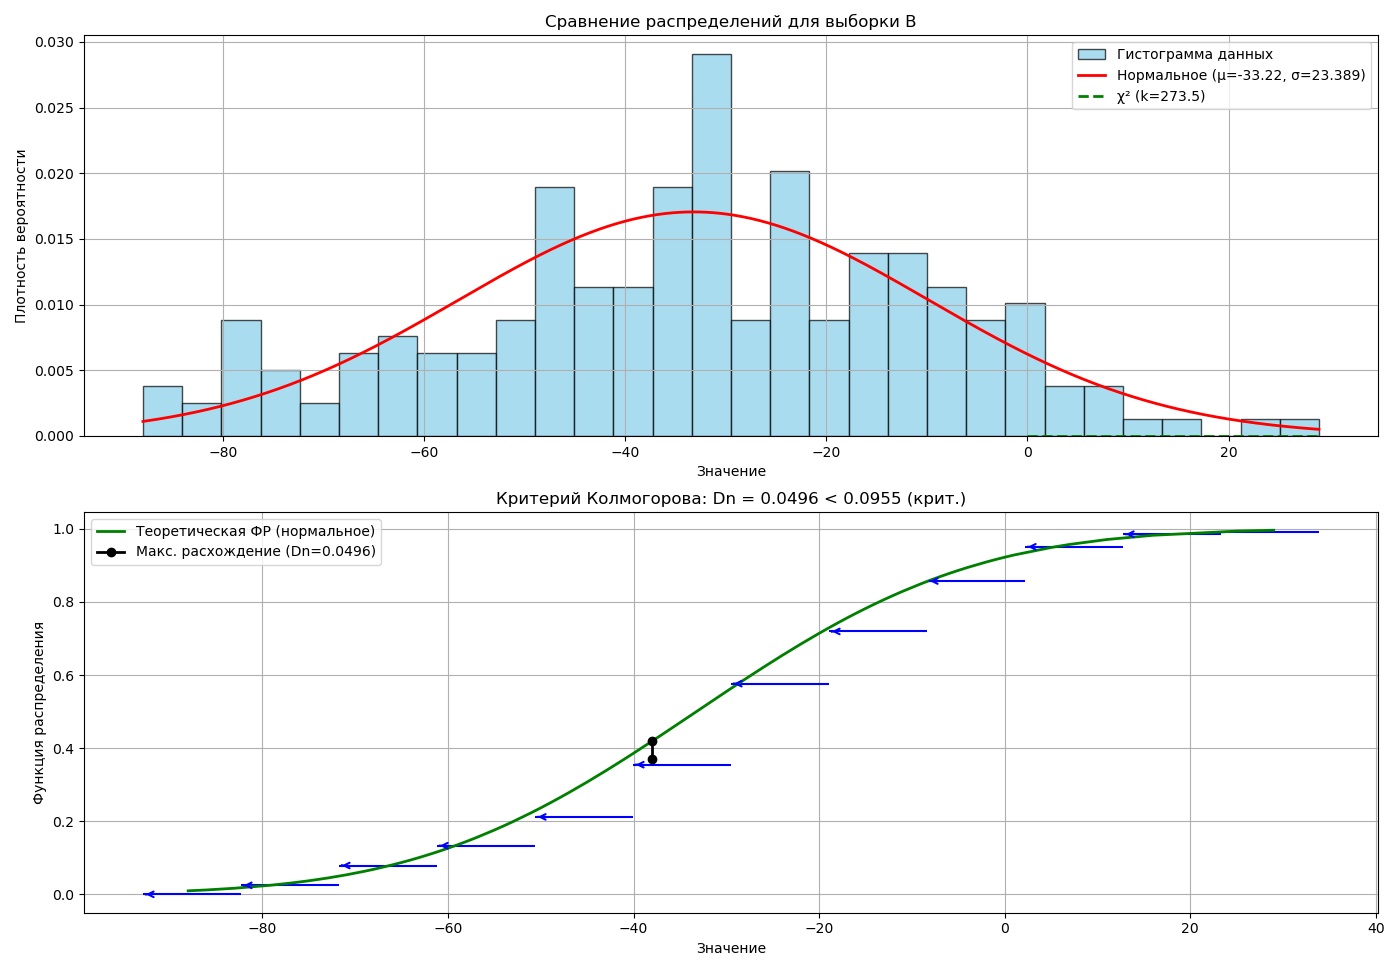
\includegraphics[scale=0.5]{normal_b.png}
\caption{График сравнения для выборки В нормального распределения}    
\end{figure}

\newpage

\subsection{Вывод о наилучшем распределении}
Нормальное распределение лучше соответствует данным, так как:
\begin{itemize}
    \item Гипотеза о нормальном распрделении не отвергается ($D_n$ < критического значения)
    \item Распределение $\chi^2$ принципиально не подходит для данных с отрицательными значениями
    \item Нормальное распрделение является естественным выбором для данных, которые могут принимать как положительные, так и отрицательные значения.
\end{itemize}

\subsection{Проверка гипотезы о среднем}
Как и прошлой секции где мы проделывали эти операции для выборки А, здесь мы также сначала выдвинем гипотезу и далее по уже известному алгоритму рассмотрим и сделаем выводы:\\
$H_0: a = a_0$, где $a_0 = [\bar{x}] - 0.5 = -34 - 0.5 = -34.5$ \\
$\bar{x} = -33.22$, $s^2 = 549.78$, $s = 23.447$, $n = 203$ \\
Найдем $Z$-статистику для сравнения с критической областью, которую найдем позже:
\[
z = \frac{\bar{x} - a_0}{s/\sqrt{n}} = \frac{-33.22 - (-34.5)}{23.447/\sqrt{203}} = 0.7768
\]
Теперь найдем критическую область из неравенства: $|z| > 1.96$ \\
Сравним нашу $Z$-статистику с критической областью и заключим: $|z| = 0.7768 < 1.96 \Rightarrow$ \textbf{гипотеза $H_0$ не отвергается}.

\subsection{Проверка гипотезы о дисперсии}
Вновь проверим гиоптезу о дисперсии, но теперь для выборки В, которую мы можем считать непрерывной. Давайте выдвинем гипотезу и рассчитаем параметр $\sigma_0^2$:
$H_0: \sigma^2 = \sigma_0^2$, где $\sigma_0^2 = [s^2] - 0.5 = 549 - 0.5 = 548.5$ \\
Как вы уже должны были догадаться, мы должны рассчитать нашу $\chi^2$ статистику, давайте сделаем это:
\[
\chi^2 = \frac{(n-1)s^2}{\sigma_0^2} = \frac{202 \times 549.78}{548.5} = 202.47
\]
Найдем критическую область:\\ 
\begin{centering}
$\chi^2 < \chi^2_{0.975}(202)$ или $\chi^2 > \chi^2_{0.025}(202)$ \\
\vspace{3mm}
$\chi^2_{0.975}(202) = 164.53$, $\chi^2_{0.025}(202) = 243.25$ \\
\end{centering}
\vspace{5mm}
Мы можем сравнить значения и получить такой вывод: $164.53 < 202.47 < 243.25 \Rightarrow$ \textbf{гипотеза $H_0$ не отвергается}.

\subsection{Проверка гипотезы о равенстве средних в двух подвыборках}
Тут уже нам не совсем повезло и количество элементов в выборке нечетное, а значит в какой-то выборке, в нашем случае давайте возьмем в первой, у нас будет меньше элементов:
$n_1 = 101$, $n_2 = 102$ \\
$\bar{x}_1 = -33.33$, $s_1^2 = 518.12$ \\
$\bar{x}_2 = -33.12$, $s_2^2 = 586.54$ \\
Проведем проверку равенства дисперсий все также через $F$-тест:
\[
F = \frac{s_1^2}{s_2^2} = \frac{586.54}{518.12} = 1.132, \quad F_{0.975}(101,100) \approx 1.48
\]
Сравним и получим, что:
$F = 1.002 < 1.43$ — дисперсии равны. \\
Объединенная дисперсию вычислим следующим образом:
\[
s_p^2 = \frac{(n_1-1)s_1^2 + (n_2-1)s_2^2}{n_1 + n_2 - 2} = \frac{100 * 518.12 + 101 * 586.54}{201} = 555.08
\]
Найдем статистику t:
\[
t = \frac{\bar{x}_1 - \bar{x}_2}{s_p \sqrt{\frac{1}{n_1} + \frac{1}{n_2}}} = \frac{-33.33 - (-33.12)}{\sqrt{555.08} * \sqrt{1/101 + 1/102}} = -0.063
\]
Найдем критическую область: $|t| > t_{0.975}(201) \approx 1.96$ \\
Тогда сравним наши значения и сделаем вывод относительно нашей гипотезы: $|t| = 0.063 < 1.96 \Rightarrow$ \textbf{гипотеза о равенстве средних не отвергается}.

\section*{Общие выводы}
\begin{enumerate}
\item Для выборки A:
\begin{itemize}
\item Лучшее распределение: Пуассон ($\lambda = 5.605$)
\item Гипотезы о среднем ($a = 5.5$) и дисперсии ($\sigma^2 = 6.5$) не отвергаются
\item При разбиении на две части средние статистически не различаются
\end{itemize}

\item Для выборки B:
\begin{itemize}
\item Лучшее распределение: нормальное ($\mu = -33.22$, $\sigma^2 = 547.07$)
\item Гипотезы о среднем ($a = -34.5$) и дисперсии ($\sigma^2 = 548.5$) не отвергаются
\item При разбиении на две части средние статистически не различаются
\end{itemize}
\end{enumerate}

\end{document}
